\section{Variable step solver}
Similar to the previous method, the \textit{convergence} of the \textit{Dormand and Prince 4(5)} solver is investigated using a test equation.
\subsection{Test Equation}
\begin{figure}[h!]
	\centering
	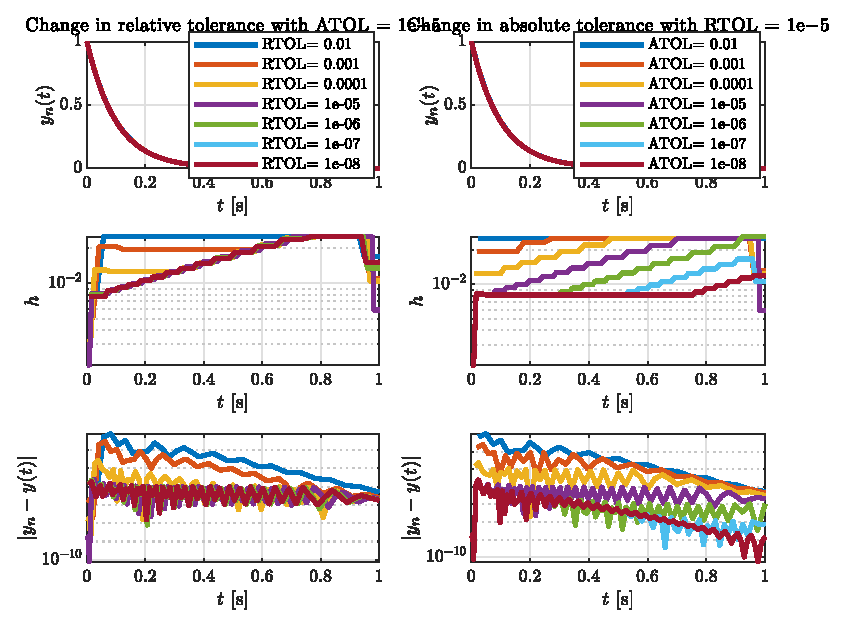
\includegraphics[width=\textwidth]{Figures/ode45_testCase.eps}
	\caption{Simulation of the test equation using the \textit{Dormand and Prince 4(5)} method with $\lambda=1$.}
	\label{fig:testode45}
\end{figure}
The consistency of the \textit{Dormand-Prince 4(5)} method is checked by using the same test equation that was used for the \textit{Euler forward} method. The test equation is given as follows:
\begin{align*}
	\textbf{Test equation: }f(t,y) &= -\lambda\,y, \quad y(0) = 1. & \textbf{Analytical solution: } & y = e^{-\lambda\,t}.
\end{align*}
Contrary to the fixed step method, the step length $h$ is varied throughout the simulation depending on the specified relative (RTOL) and absolute (ATOL) tolerances. 

The simulation results of the test equation are presented in \prettyref{fig:testode45}. From the figure, it is clear that by varying only the relative tolerance (RTOL), there is no significant difference in the error signal ($e(t_N) = |y_N - y(t_N)|$) at time $t = t_N$. This is because $h$ at $t = t_N$ for different RTOL are similar. However, varying the absolute tolerance (ATOL), it is clear that as $h\rightarrow0,\ |y_n - y(t)| \rightarrow0$. At time $t = t_{N-1}$ there is a sudden change in $h$ possibly be due to numerical rounding errors. Therefore time $t_{N-1}$ was considered for consistency check. According to the fundamental convergence theorem, the solver is convergent. Furthermore, from the figure it can be concluded RTOL controls the rate of change of $h$ and ATOL controls the absolute value of $h$

The average step size for convergence in the \textit{Dormand and Prince 4(5)} method have larger $h$ than the \textit{Euler forward} method. At the same time, the error in \textit{Dormand and Prince 4(5)} is lower than the error in the \textit{Euler forward}. This indicates the \textit{Dormand and Prince 4(5)} is a higher order method than the \textit{Euler forward}. 

\subsection{Motor equation}
\begin{figure}[t!b!]
	\centering
	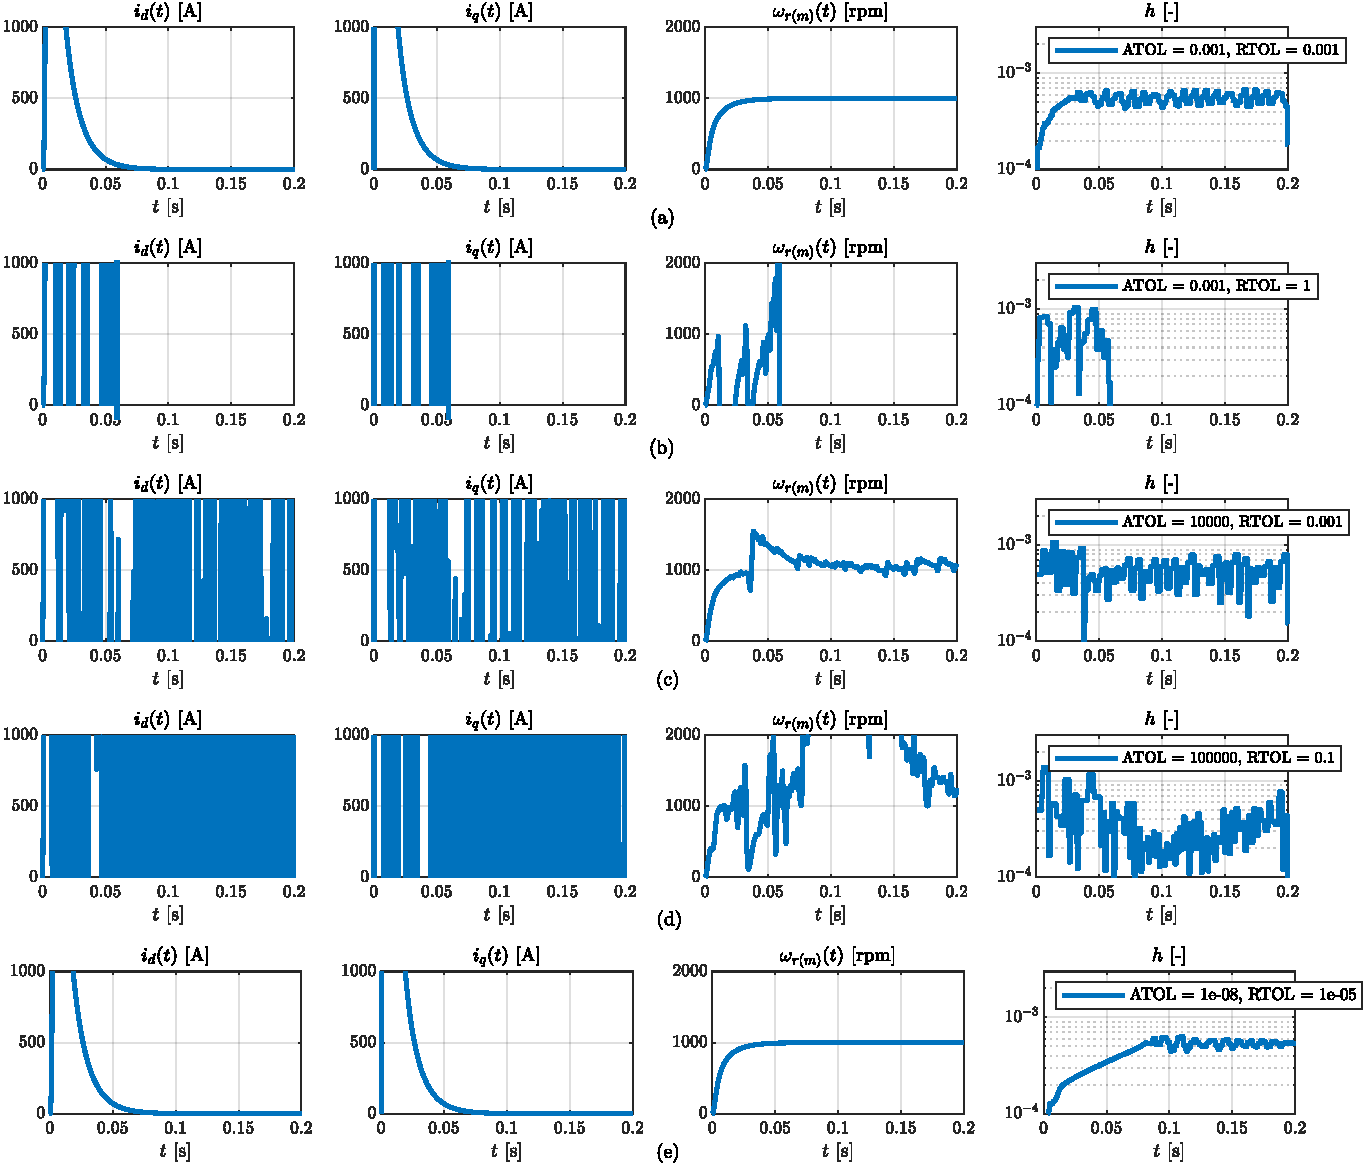
\includegraphics[width=\textwidth]{Figures/ef_MotorCase_ode45_Atol_Rtol.pdf}
	\caption{Simulation of the PMSM using Euler forward method with $\vd=\vq=800\,$V at different absolute (ATOL) and relative tolerances (RTOL). (a) ATOL = 0.001 RTOL = 0.001, (b) ATOL = 0.001 RTOL = 1, (c) ATOL = 1e4 RTOL = 0.001, (d) ATOL = 1e5 RTOL = 0.1, and (e) ATOL = 1e-8 RTOL = 1e-5}
	\label{fig:EMresOde45}
\end{figure}
\prettyref{fig:EMresOde45} presents the simulation results of a PMSM using the \textit{Dormand and Prince 4(5)} method. The figure shows the states (dynamic variables) \id, \iq and \wm as a function of time at different ATOL and RTOL. \prettyref{fig:EMresOde45}(a) presents the simulation results considering ATOL = RTOL = 0.001 and it is clear the dynamic variables \id, \iq, and \wm, converge implying the stability of both the ODE and the solver. Furthermore, the average set size is about 0.5e-3\,s and a deviation of 0.1e-3\,s. Moreover, at $t < 0.5$\,s the step size increases gradually from lower than 1e-4\,s to about 0.5e-3\,s. \prettyref{fig:EMresOde45}(b) presents simulation results with ATOL = 0.001 and RTOL = 1. From the figure it is clear that the simulation does not converter after $t \approx 0.05$\,s and the solutions is $\infty$. $h$ at $t_1$ (1\textsuperscript{st} step) is lower than 1e-4. However, just after a few steps, $h$ increases to 0.9e-3 as a consequence, the solver is does not converge. \prettyref{fig:EMresOde45}(c) and \prettyref{fig:EMresOde45}(d) presents simulation results with ATOL = 1e4 and RTOL = 0.001, and ATOL = 1e5 and RTOL = 0.1, respectively. From the figure it is clear that in both cases $h$ varies between 1e-4 and 1e-3\,s throughout the simulation and as a result, the simulation is although bounded, is not stable, ex: the drastic change in \wm at $t = 0.035$\,s indicates the instability of the solver. \prettyref{fig:EMresOde45}(e) presents simulation results with ATOL = 1e-8 and RTOL = 1e-5 and from the figure it is clear that the simulation converges. Furthermore, $h$ increases gradually to 0.5e-5\,s at $t = 0.75$\,s due to very low RTOL. 

%From the figure, although not straightforward, it can be seen that with lower $h\rightarrow0$ all the states converges to a constant value. This implies that that % the solver is 0\textit{-stable}. Furthermore, it is also clear that 
% the ODE system is stable for ATOL$\geq10$. 
%From the figure it is clear with lower $h\rightarrow0$. all the states converges to a constant value. This implies that that the solver is \textit{0-stable}. Furthermore, it is also clear that the ODE system is also stable. 
%
%In the previous section it was verified the \textit{convergence} of the numerical method. Therefore, it is observed that the simulated results with $h \leq 1\text{e}-4$ gives the a solution that is very close to the true solution to the ode system.

%the order of the system is calculated and presented in the table below:
%\begin{table}[h!]
%	\centering
%	\begin{tabular}{c|c|c|c}
%		TOL & $h_n$ & $|y_n - y(t)|$ & $p$ \\
%		\hline
%		0.1 & 0.07 & 5.82e-7 & \\
%		0.01 & 0.09 &5.89e-7 & 1.23\\
%		0.001 & 0.06 & 3.62e-7 & 1.02 \\
%		0.0001 & 0.06 & 8.18e-8 & 4.38\\
%		1e-5 & 0.03 & 9.37e-9 & 4.6 \\
%		1e-6 & 0.02 & 9.91e-10 & 6.67 \\		
%		1e-7 & 0.02 & 1.01e-10 & 9.13 \\
%	\end{tabular}
%\end{table}\\
%From the table and the figure, it is clear that, as $h\rightarrow0,\ |y_n - y(t)| \rightarrow0$. Therefore, according to the fundamental convergence theorem, the solver is convergent of order $p$. 